\begin{figure}
\begin{columns}
\begin{column}{0.05\textwidth}
\begin{subfigure}[b]{\textwidth}
\caption{}
\label{fig:natural}
\end{subfigure}
\end{column}
\begin{column}{0.27\textwidth}
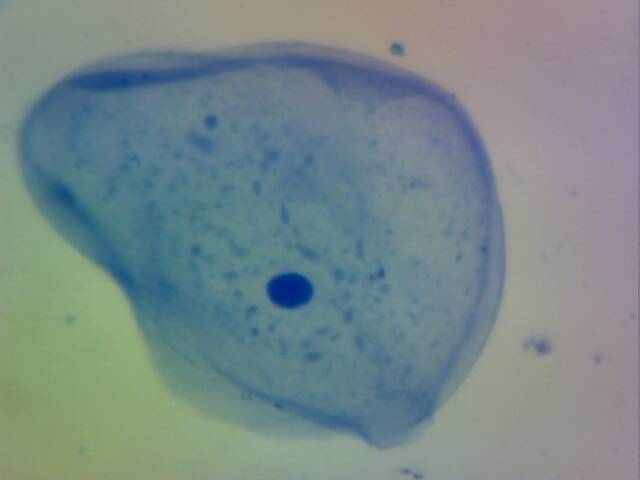
\includegraphics[width=\textwidth]{cheek_cell}
\end{column}
\begin{column}{0.07\textwidth}

\includegraphics[width=\textwidth]{arrow}
\end{column}
\begin{column}{0.27\textwidth}
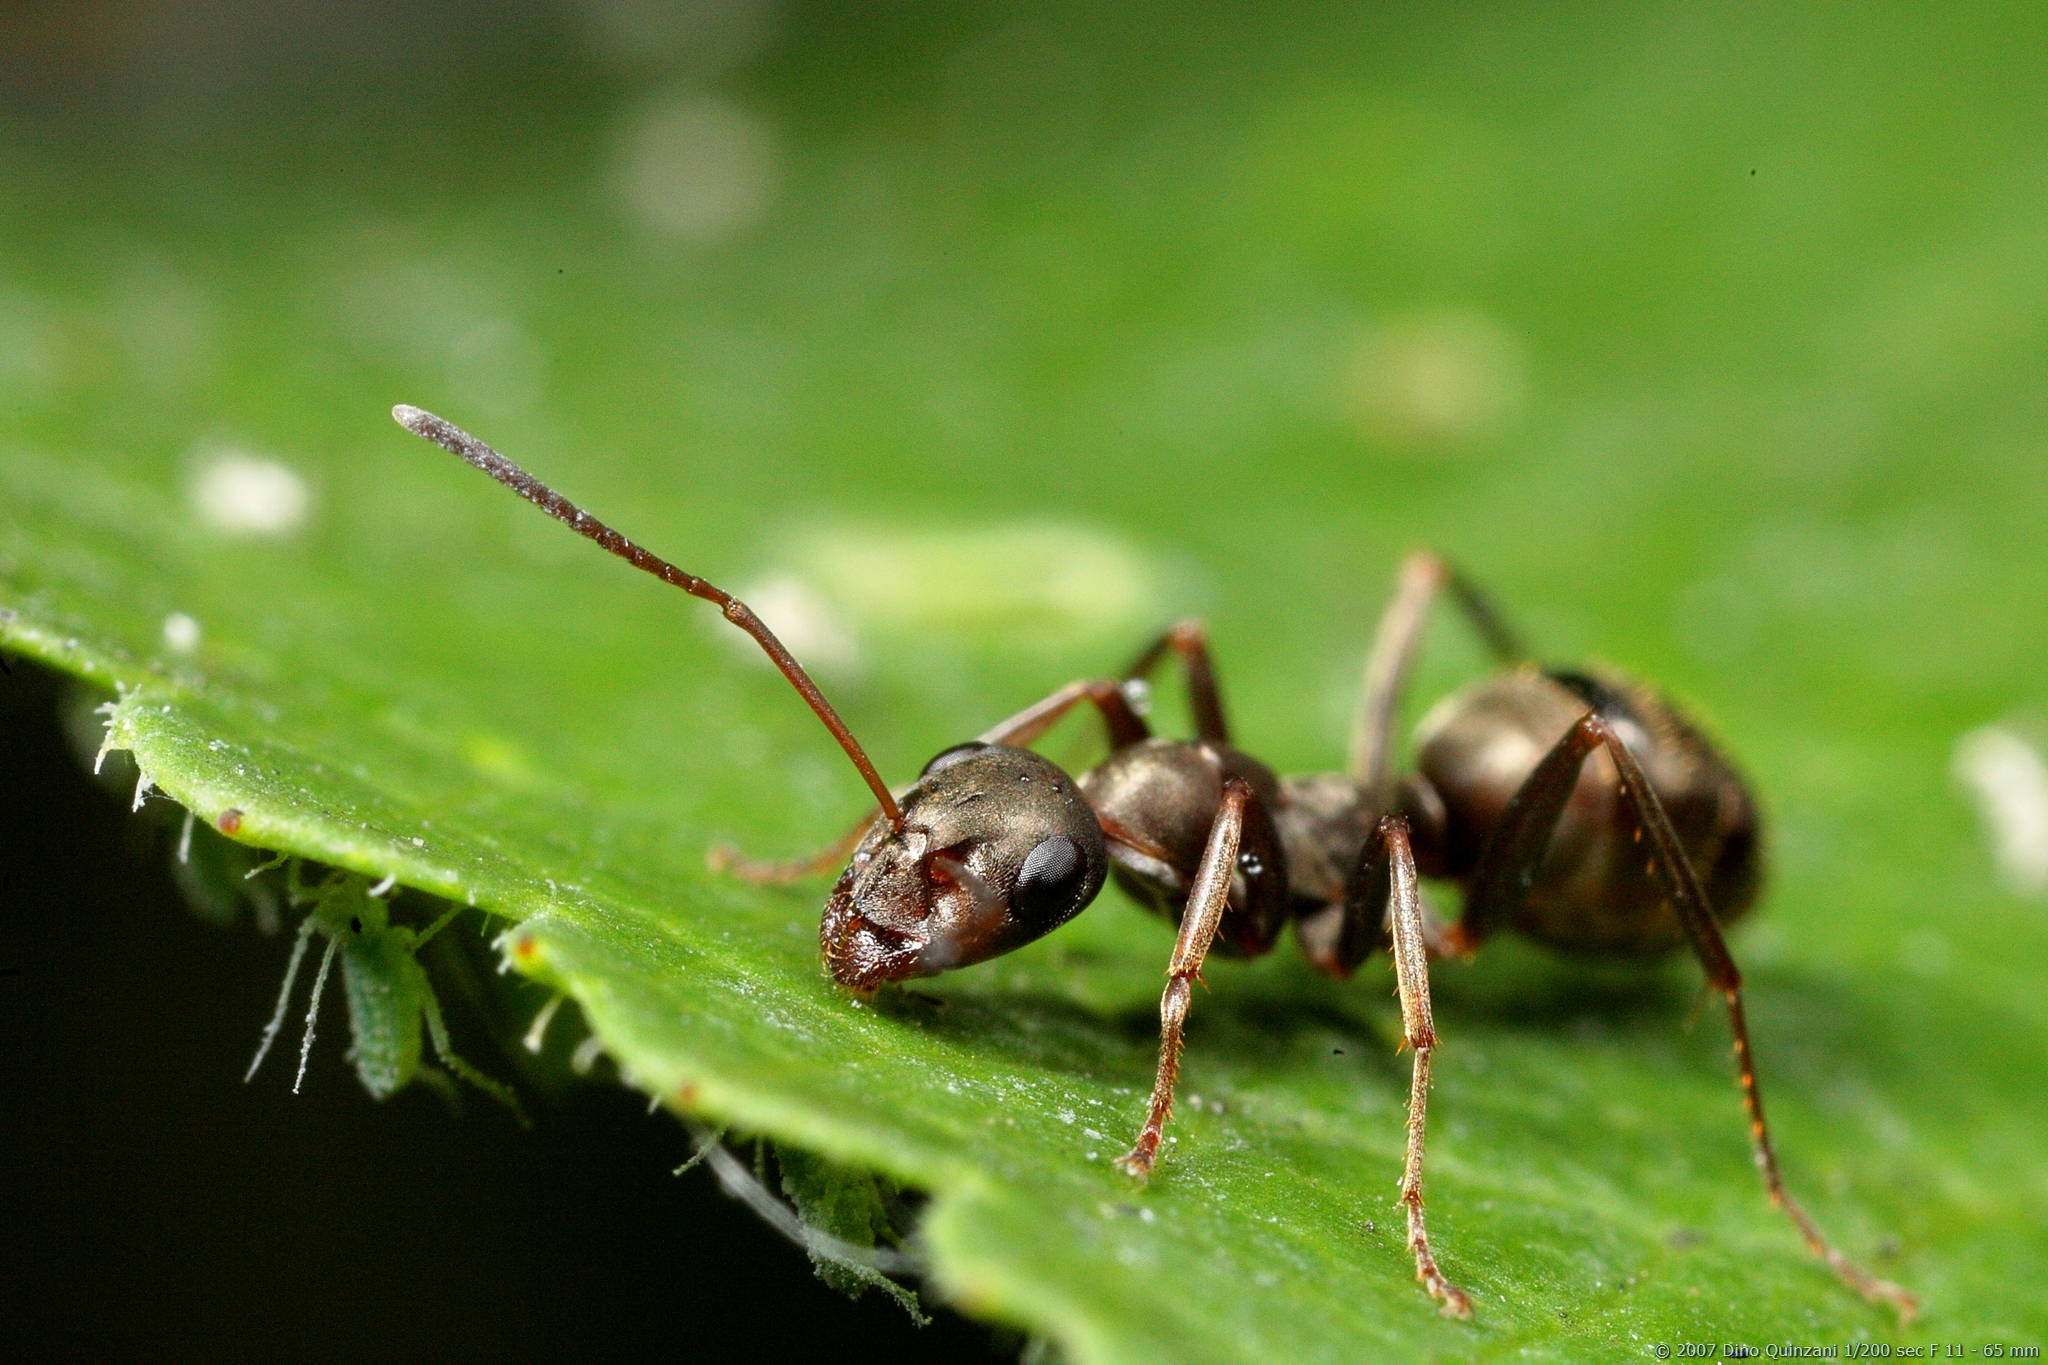
\includegraphics[width=\textwidth]{ant}
\end{column}
\begin{column}{0.07\textwidth}

\includegraphics[width=\textwidth]{arrow}
\end{column}
\begin{column}{0.27\textwidth}
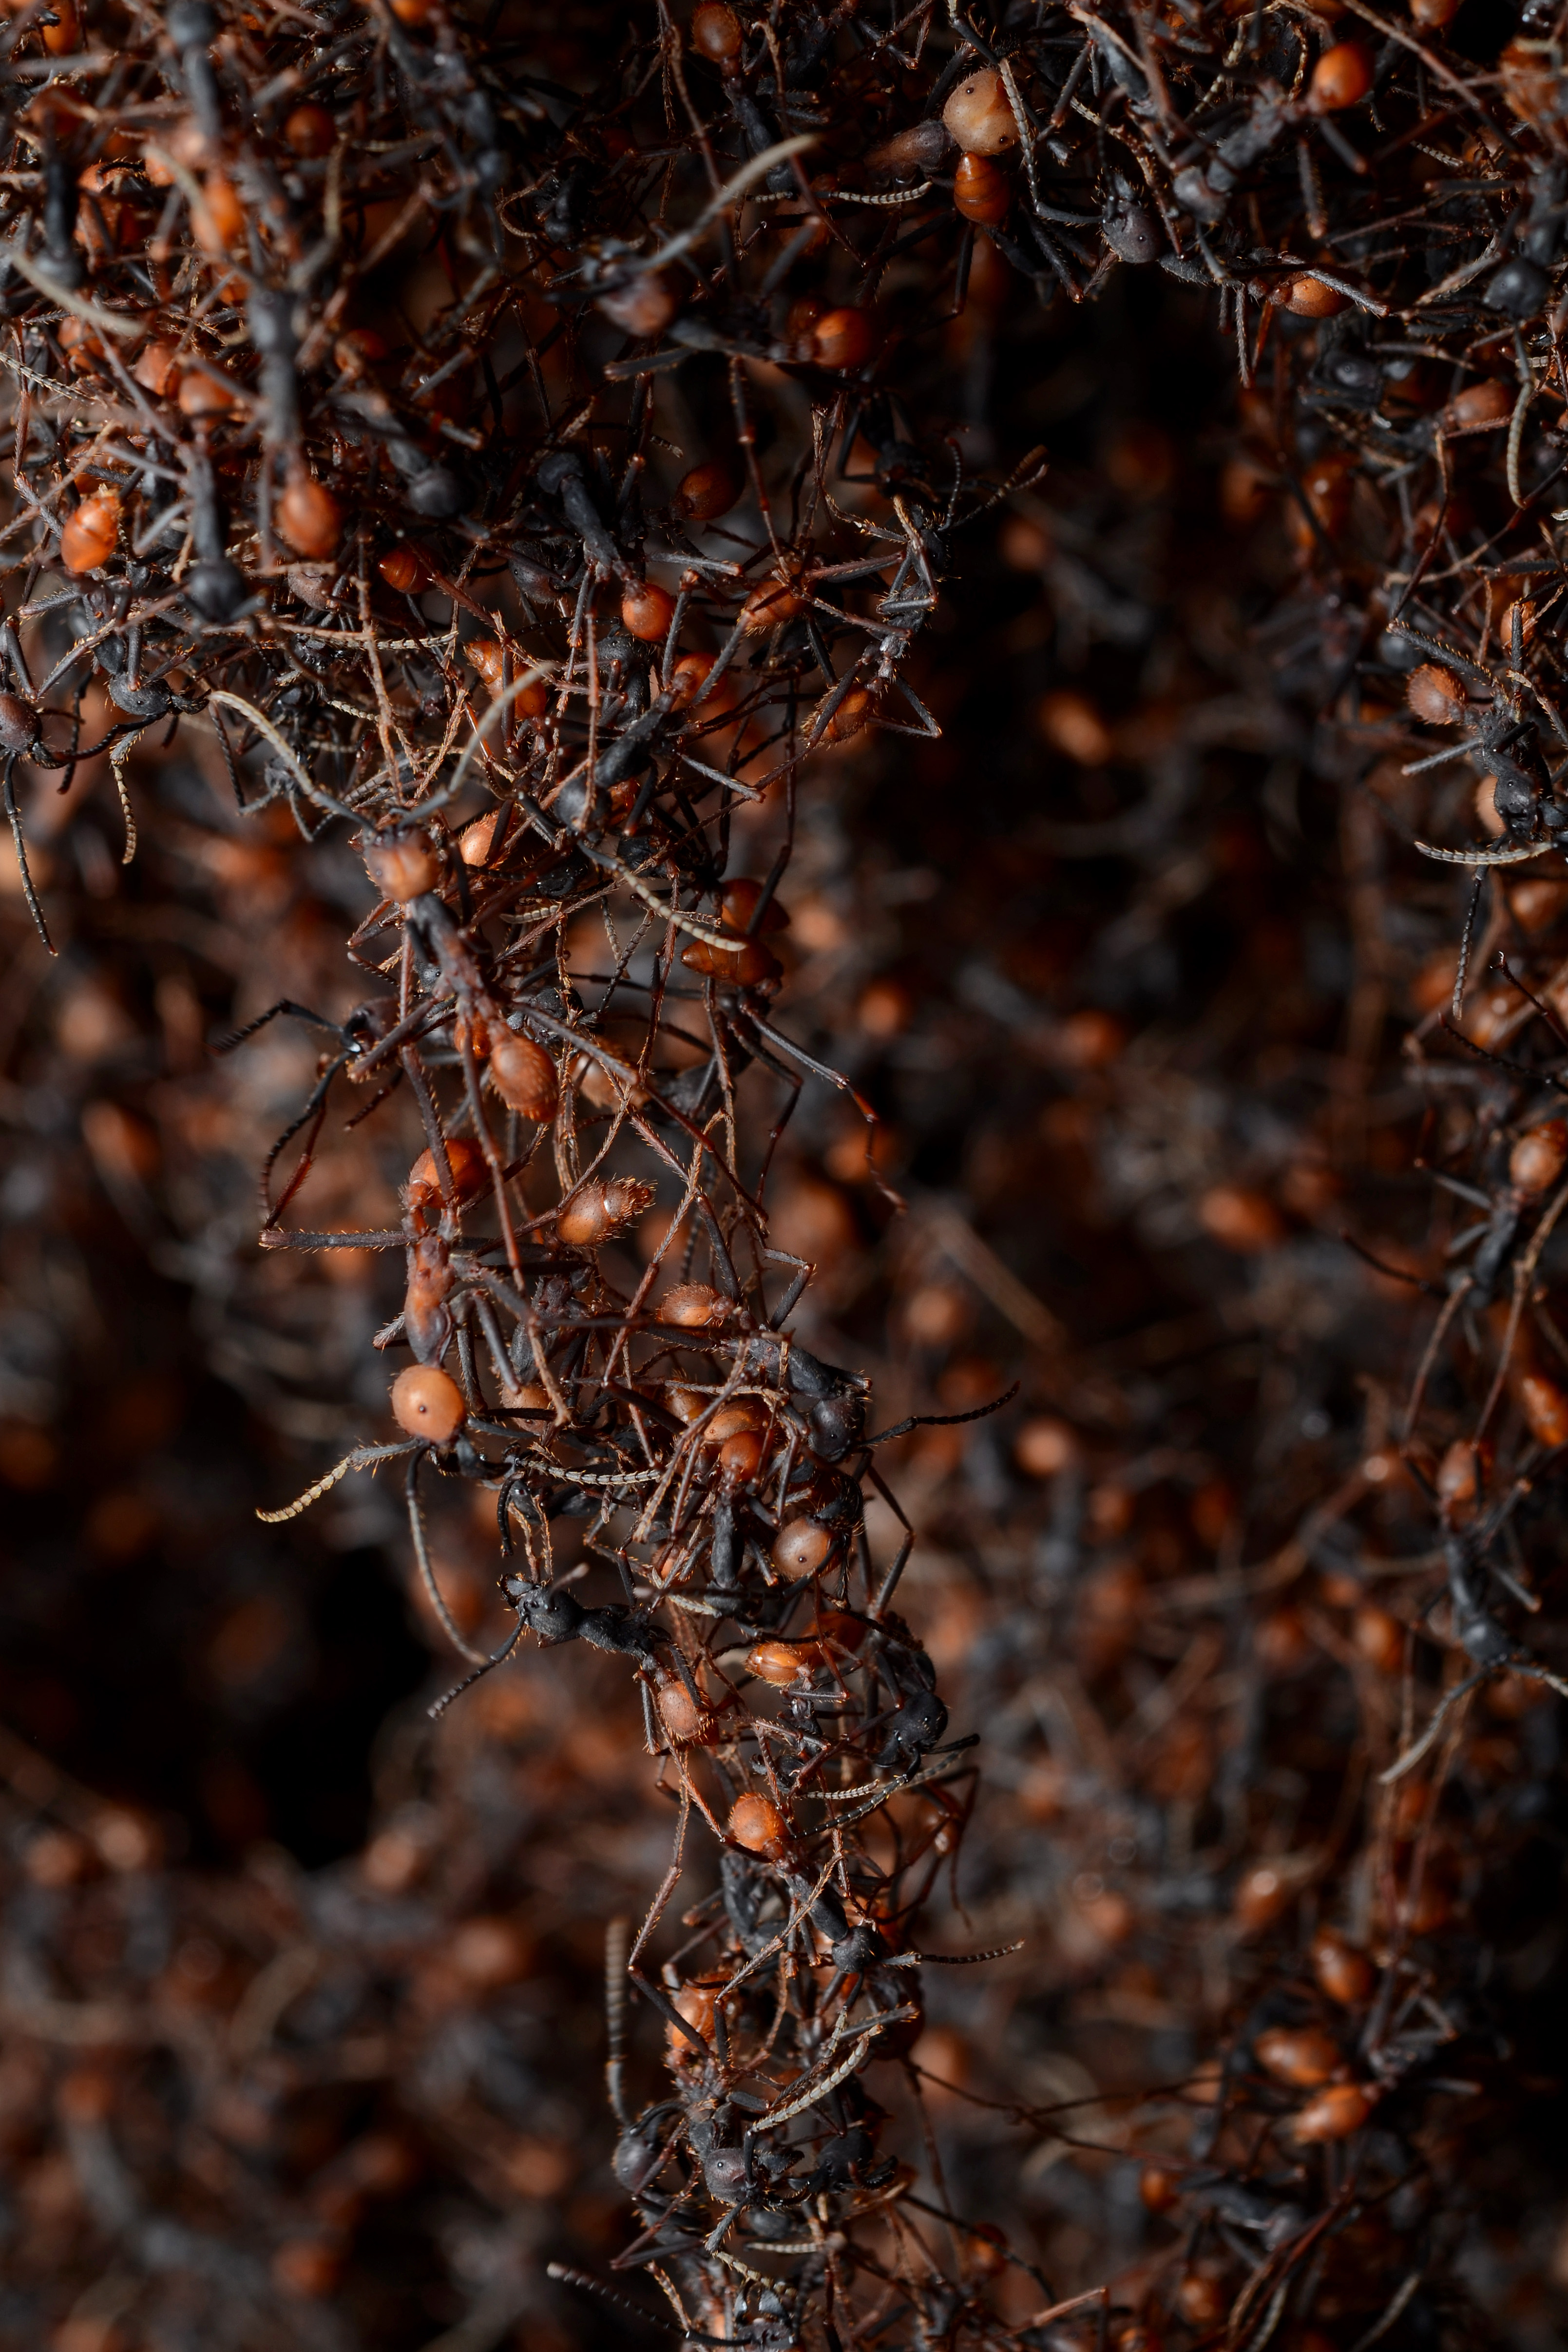
\includegraphics[angle=270, width=\textwidth]{ant_bridge}
\end{column}
\end{columns}
\vspace{1ex}
\begin{columns}
\begin{column}{0.05\textwidth}
\end{column}
\begin{column}{0.27\textwidth}
\centering
cell {\tiny\cite{clare_and_ben_2017}}
\end{column}
\begin{column}{0.07\textwidth}
\end{column}
\begin{column}{0.27\textwidth}
\centering
ant {\tiny\cite{quinzani_2008}}
\end{column}
\begin{column}{0.07\textwidth}
\end{column}
\begin{column}{0.27\textwidth}
\centering
ant colony {\tiny\cite{gallice_2011}}
\end{column}
\end{columns}
\begin{columns}
\begin{column}{0.05\textwidth}
\end{column}
\begin{column}{0.27\textwidth}
\centering
\end{column}
\begin{column}{0.07\textwidth}
\end{column}
\begin{column}{0.27\textwidth}
\centering
(clump)
\end{column}
\begin{column}{0.07\textwidth}
\end{column}
\begin{column}{0.27\textwidth}
\centering
(clump of clumps)
\end{column}
\end{columns}
\vspace{2ex}
\begin{columns}
\begin{column}{0.05\textwidth}
\begin{subfigure}[b]{\textwidth}
\caption{}
\label{fig:simulated}
\end{subfigure}
\end{column}
\begin{column}{0.27\textwidth}

\includegraphics[width=\textwidth]{cell}
\end{column}
\begin{column}{0.07\textwidth}
{\Large$\underset{\phantom{\checkmark}}{\overset{\checkmark}{
\includegraphics[width=\textwidth]{arrow}}}$}
\end{column}
\begin{column}{0.27\textwidth}
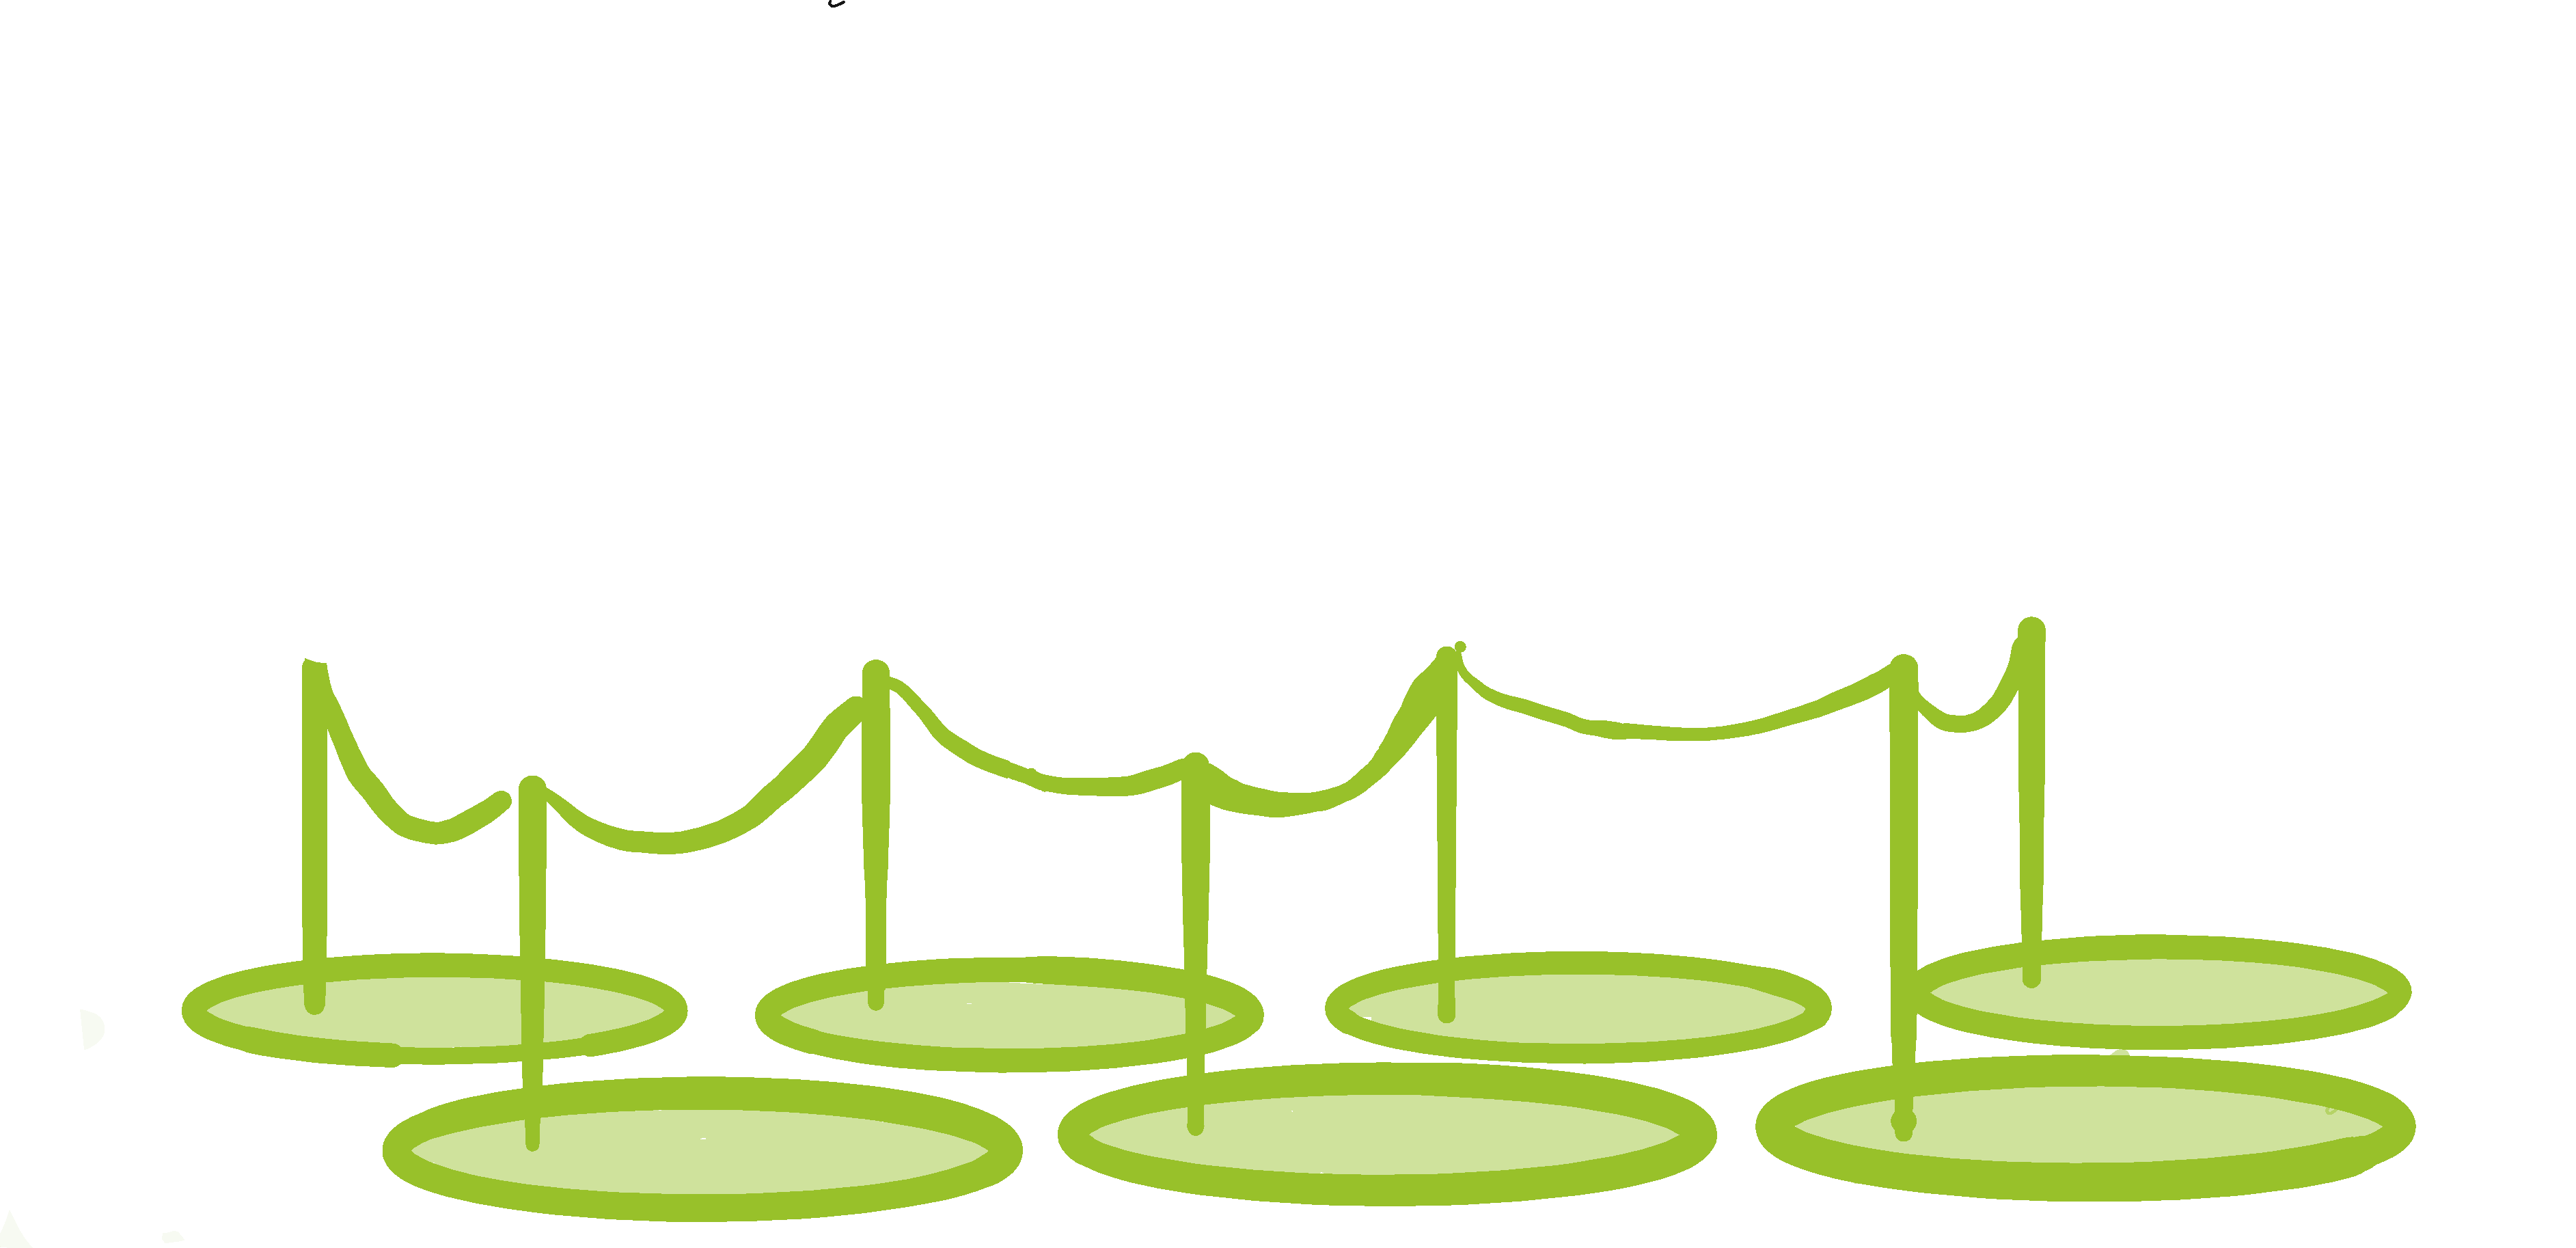
\includegraphics[width=\textwidth]{clump}
\end{column}
\begin{column}{0.07\textwidth}
{\Large$\underset{\phantom{?}}{\overset{\only<1,2>{?}\only<3>{\phantom{?}}}{
\includegraphics[width=\textwidth]{arrow}}}$}
\end{column}
\begin{column}{0.27\textwidth}
\centering
\only<1,2>{\Large ?} \only<3>{\Large \phantom{?}}
\includegraphics[width=\textwidth]<2>{clumps}
\includegraphics[width=\textwidth]<3>{clump_of_clumps}
\end{column}
\end{columns}
\vspace{1ex}
\begin{columns}
\begin{column}{0.05\textwidth}
\end{column}
\begin{column}{0.27\textwidth}
\centering
cell
\end{column}
\begin{column}{0.07\textwidth}
\end{column}
\begin{column}{0.27\textwidth}
\centering
clump
\end{column}
\begin{column}{0.07\textwidth}
\end{column}
\begin{column}{0.27\textwidth}
\centering
\only<3>{\phantom{(}}\only<1,2>{(}clump of clumps\only<1,2>{)}\only<3>{\phantom{)}}
\end{column}
\end{columns}
\vspace{2ex}
\caption{Analogy between (\subref{fig:natural}) natural and (\subref{fig:simulated}) simulated hierarchical fraternal transitions of individuality.}

\end{figure}
